% Bisognano--Wichmann / Unruh.
% (a) Euclidean (x, t_E) plane: the t=0 slice is the horizontal axis, R = right
%     half-line, L = left half-line; the Euclidean boost angle eta_E rotates
%     about the horizon point rho = 0 with period 2 pi (R -> L at eta_E = pi).
% (b) Local Unruh temperature on the t = 0 slice of R, T(x) = 1/(2 pi x)
%     (hbar = c = k_B = 1), plotted from the formula.
% Included at 0.78\textwidth (5.07in); drawn at ~1:1.
\documentclass[tikz,border=3pt]{standalone}
\usepackage[T1]{fontenc}
\usepackage{lmodern}
\usepackage{amsmath,amssymb}
\usepackage{xcolor}
\usetikzlibrary{arrows.meta}

\definecolor{ruleblue}{HTML}{2b6cb0}
\definecolor{rulegold}{HTML}{b7791f}
\definecolor{rulered}{HTML}{c0392b}
\definecolor{axisgray}{HTML}{8a8f98}

\begin{document}
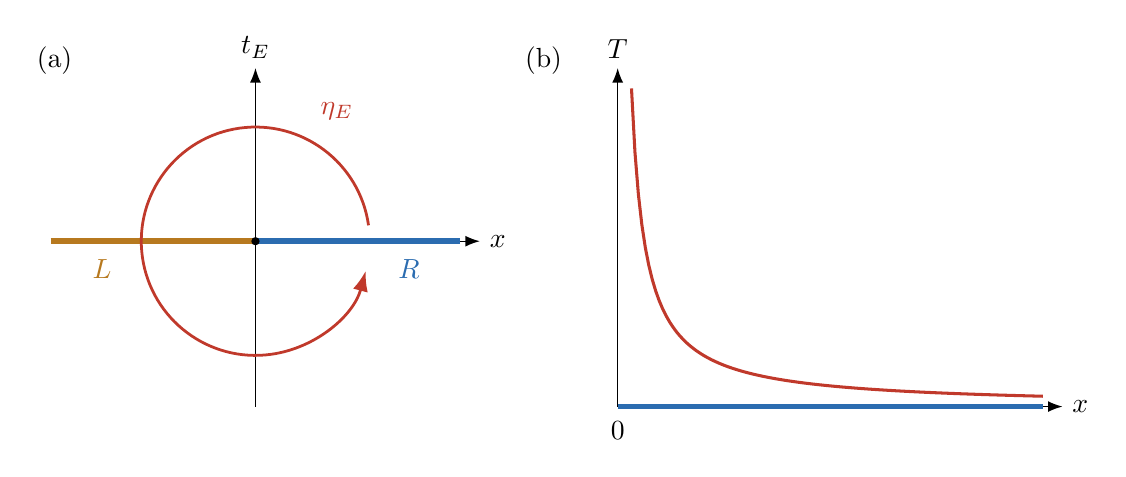
\begin{tikzpicture}[>=Latex]
  % ---------------- (a) Euclidean plane ----------------
  \begin{scope}
    \draw[->, line width=0.5pt] (0,-2.1) -- (0,2.2) node[above] {$t_E$};
    \draw[rulegold, line width=2pt] (-2.6,0) -- (0,0);
    \draw[ruleblue, line width=2pt] (0,0) -- (2.6,0);
    \draw[->, line width=0.5pt] (2.6,0) -- (2.85,0) node[right] {$x$};
    \node[ruleblue, below=3pt] at (1.95,0) {$R$};
    \node[rulegold, below=3pt] at (-1.95,0) {$L$};
    % circle of fixed rho, and the Euclidean rotation
    \draw[-{Latex[length=2.6mm]}, rulered, line width=1pt]
      (8:1.45) arc[start angle=8, end angle=345, radius=1.45];
    \node[rulered] at (58:1.95) {$\eta_E$};
    \fill (0,0) circle (1.5pt);
    \node[anchor=north west] at (-2.9,2.6) {(a)};
  \end{scope}

  % ---------------- (b) T(x) on the t = 0 slice ----------------
  \begin{scope}[xshift=4.6cm, yshift=-2.1cm]
    \def\sx{1.35}  % cm per unit x
    \def\sy{3.3}   % cm per unit T
    \draw[->, line width=0.5pt] (0,0) -- (0,4.3) node[above] {$T$};
    \draw[ruleblue, line width=2pt] (0,0) -- ({4*\sx},0);
    \draw[->, line width=0.5pt] ({4*\sx},0) -- ({4*\sx+0.25},0) node[right] {$x$};
    \draw[rulered, line width=1.1pt, domain=0.13:4, samples=120, variable=\x]
      plot ({\x*\sx}, {\sy/(2*pi*\x)});
    \node[below=2pt] at (0,0) {$0$};
    \node[anchor=north west] at (-1.3,4.7) {(b)};
  \end{scope}
\end{tikzpicture}
\end{document}
